\hypertarget{group__RXSPEC}{\section{Guarantees}
\label{group__RXSPEC}\index{Guarantees@{Guarantees}}
}
Collaboration diagram for Guarantees\+:\nopagebreak
\begin{figure}[H]
\begin{center}
\leavevmode
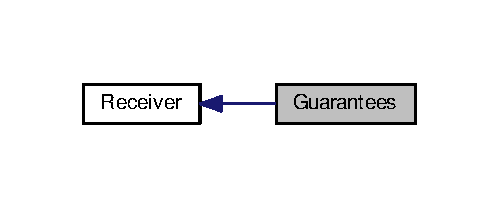
\includegraphics[width=240pt]{group__RXSPEC}
\end{center}
\end{figure}
This is a summary of automatic tests that are done against the receiver module to guarantee that the module behaves according to the requirements set forth below.


\begin{DoxyItemize}
\item R\+X should output data on 16 channels. If hardware supports less then rx should output failsafe values on the remaining channels. If supplied channel is out of range then rx should output {\itshape midrc}.
\item On startup all receiver channels should return failsafe values. As new channels are connected rx will return the received values. However as any of the channels lose signal rx should hold the value for a timeout and then mark the rx as not heathy and return failsafe for that single channel. As the channel is connected again, rx should become heathy. R\+X should report that it has signal until all channels are lost.
\item Upon signal loss (all channels first valid then invalid) all channels should be outputting failsafe values.
\item Each channel shall have configurable failsafe that can output one of three alternatives\+: 1) auto\+: all channels are set to midrc except throttle. 2) hold\+: holds old channel information. 3) set\+: failsafe returnes a user configurable value. For safety reasons, non-\/aux channels should only support A\+U\+T\+O mode.
\item Receiver shall support channel remapping using a string that specifies ordering of the channels. Incoming signal shall be mapped from supplied configuration into standard \char`\"{}\+A\+E\+R\+T12345678abcdefgh\char`\"{} channel ordering.
\item R\+X outputs shall be represented by microsecond interval in range of rx\+\_\+min\+\_\+usec$\ast$ to {\itshape rx\+\_\+max\+\_\+usec}. If any inputs are outside of this range then they should be properly constrianed. 
\end{DoxyItemize}